\documentclass[prl,twocolumn,floatfix,superscriptaddress,aps]{revtex4-2}

\usepackage{graphicx}
\usepackage{bm}

\usepackage{amsmath}
\usepackage{units}

\usepackage{hyperref}
\hypersetup{colorlinks=true, citecolor=blue, urlcolor=blue, linkcolor=blue}

% \usepackage{todonotes}

\renewcommand{\vec}[1]{\boldsymbol{#1}}
\newcommand{\com}[1]{{\color{magenta} #1}}
\newcommand{\rework}[1]{{\color{blue}{#1}}}


\begin{document}
\title{Magnetic dichroism in darkfield UV photoemission electron microscopy}
\author{Maximilian Paleschke}
\author{David Huber}
\author{Friederike Wührl}
\affiliation{Institute of Physics, Martin Luther University Halle-Wittenberg, D-06099 Halle (Saale), Germany}

\author{Cheng-Tien Chiang}
\affiliation{Institute of Atomic and Molecular Sciences, Academia Sinica, Taipei, Taiwan}

\author{Frank O. Schumann}
\affiliation{Max-Planck-Institut f\"{u}r Mikrostrukturphysik, 06120 Halle, Germany}

\author{Jürgen Henk}
\author{Wolf Widdra}
\affiliation{Institute of Physics, Martin Luther University Halle-Wittenberg, D-06099 Halle (Saale), Germany}

\email{wolf.widdra@physik.uni-halle.de}

\date{\today}

\begin{abstract}
    Photoemission electron microscopy (PEEM) has evolved into an indispensable tool for structural and magnetic characterization of surfaces at the nanometer scale. In strong contrast to synchrotron-radiation-based X-ray PEEM as a leading method for element-specific magnetic properties via magnetic circular dichroism (MCD), laboratory ultraviolet (UV) PEEM has seen limited application with much smaller dichroism effects for in-plane magnetization. Here we introduce darkfield PEEM as a novel approach to enhance MCD contrast in threshold photoemission, enabling efficient MCD imaging with significantly enhanced contrast by order-of-magnitude for Fe(001). This advancement paves the way for
    MCD imaging on femtosecond timescales using modern lasers. The experimental results will be quantitatively benchmarked against advanced relativistic photoemission calculations.
\end{abstract}

\pacs{}

\maketitle
% Paragraph headings may be deleted in the final version .
%\paragraph{Introduction.} 
Ultrafast spin and magnetization dynamics are exciting and rapidly growing fields in condensed matter physics with promising implications for both future research and device applications. Ultrafast imaging of magnetic domains on the micrometer scale is well established utilizing all-optical methods, as e.g.\ Kerr microscopy. On the nanometer scale, however, electron microscopy is the method of choice due to the electrons' short de Broglie wavelength. 

Magnetic circular dichroism (MCD) provides the contrast mechanism used for imaging magnetic domains in photoelectron emission microscopy (PEEM). The intensity recorded for a particular domain changes with the helicity of the incident radiation, thereby producing magnetic contrast without need for explicitly detecting the electron spin. By tuning the incident X-ray radiation to a magnetic core level absorption edge, substantial and element-specific MCD asymmetries have been reported. With the wide availability of tunable synchrotron radiation, this technique of XMCD-PEEM is well established for magnetic domain imaging on the nanometer scale \cite{kuch15}. However, the pulse length of synchrotron radiation of typically $\unit[30-50]{ps}$ renders XMCD-PEEM unsuitable on ultrafast timescales. Replacing the incident X-ray radiation by ultrashort laser pulses would solve this issue straightforwardly and allow for pump-probe experiments on the timescale of a  few femtoseconds. In addition, experiments can be performed in the laboratory with UV laser sources, which excite electrons close to the Fermi level to energies slightly above the escape threshold. However, reported MCD contrasts are quite small in threshold photoemission \cite{marx2000}, especially for in-plane magnetization. Obviously, magnetic contrast needs to be increased for domain imaging with ultrashort laser pulses.

As we demonstrate here, the concept of darkfield PEEM in threshold photoemission allows efficient MCD imaging with an order-of-magnitude enhanced MCD contrast for in-plane magnetization. It paves the way for MCD imaging on femtosecond timescales with modern UV laser sources. Darkfield PEEM imaging uses an aperture for photoelectron momentum selection in the back focal plane of the electron imaging column prior to forming the real-space image. We will demonstrate this for the in-plane magnetic structure at the Fe(001) surface and compare quantitatively the experimental results with fully relativistic photoemission calculations.

Following initial reports of magnetic dichroism in UV photoemission and its theoretical description in the 1990s \cite{schneider1991,henk1996,feder1996}, Marx \textit{et al.}\ reported the first observation of magnetic dichroism in threshold PEEM in 2000 \cite{marx2000}. This study of polycrystalline Fe revealed an asymmetry in magnetic linear dichroism of $\unit[0.37]{\%}$. Subsequent spectroscopic studies confirmed the presence of both circular and linear dichroism in various ferromagnetic materials. Building on Marx's experimental work, Nakagawa \textit{et al.}\ studied Ni films adsorbed with Cs and discovered significant asymmetries of up to $\unit[12]{\%}$ in circular dichroism PEEM for out-of-plane magnetized domains \cite{nakagawa2007,nakagawa2009,nakagawa2012}. This work also demonstrated the feasibility of using pulsed laser light for dichroism imaging. However, due to the limited photon energy range of common optical laser setups, Cs remained necessary in most photoemission experiments in order to reduce the work function \cite{kronseder2011, meier2017}, although PEEM studies using a deep-UV laser with a photon energy of $\unit[7]{eV}$ have been reported \cite{zhao2019}. 

The theoretical framework for valence-band dichroism was primarily developed in the 1990s and early 2000s \cite{tamura1987, feder1996,henk1996,kuch1996a,feder1998,venus1994,venus1997,kuch2001} and was bolstered by pioneering experiments \cite{venus95, hild2008, hild2009, hild2010}. It is based on calculating the relativistic electronic  structures in conjunction with a theoretical description of the photoemission process. 
The extension of this description to threshold photoemission predicted that experimentally accessible magnetic dichroism levels are expected \cite{feder1998}. 


% \paragraph{Conceptual basis.} 
For a simplified conceptual approach, we consider a surface with fourfold symmetry, as e.g. the (001) fcc or bcc surfaces with magnetic easy axes along one of the four [100] 
or [110] 
directions. Let us assume light incidence along the surface normal (Fig.~\ref{fig:symmetry} for $\theta = 0$). The photoemission intensity of electrons detected with off-normal wavevector $\vec{k}$ depends then on the helicity, $\sigma_{+}$ or $\sigma_{-}$, of the incident circular polarized laser radiation and on the two orientations $\pm M$ of the in-plane magnetization in a selected domain, yielding four intensities $I_{\vec{k}}(\sigma_{\pm}, \pm M)$ (shortened $I_{\pm \pm}$). The latter intensities are combined into the total intensity
\begin{align}
    I & \equiv I_{+ +} + I_{+ -} + I_{- +} + I_{- -}. 
\end{align}
In order to disentangle the two main contrast mechanisms, we define appropriate asymmetries \cite{henk1998},
\begin{subequations}
\begin{align}
    A_{\mathrm{pol}} & \equiv \left[ \left( I_{+ +} + I_{+ -} \right) - \left( I_{- +} + I_{- -} \right) \right] / I,
    \label{eq:Apol}
    \\
    A_{\mathrm{ex}} & \equiv \left[ \left( I_{+ +} + I_{- -} \right) - \left( I_{+ -} + I_{- +} \right) \right] / I.
    \label{eq:Aex}
\end{align}    
\end{subequations}
In the polarization asymmetry $A_{\mathrm{pol}}$ the magnetization's orientation is averaged out; it thus encodes contrast due to the light's helicity, as if the domain were nonmagnetic. Contrast due to the exchange splitting is quantified by the exchange asymmetry $A_{\mathrm{ex}}$, in which one averages over the mutual orientations of helicity and magnetization. Note that the \emph{chiral geometry} for photoelectrons with \emph{off-normal} wavevector $\vec{k}$ outside the scattering plane results in magnetic dichroism and, hence, in magnetic contrast.

\begin{figure}
    \centering
    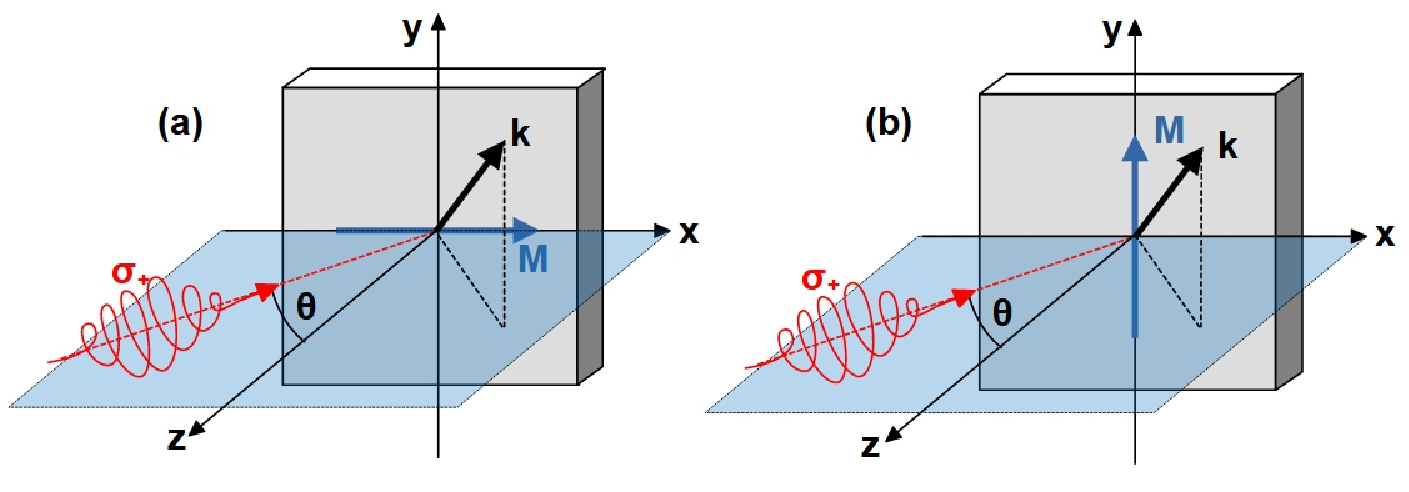
\includegraphics[width = \columnwidth]{symmetry}
    \caption{Symmetry analysis. A circular polarized laser pulse (orange, with helicity $\sigma_{+}$ impinges onto a magnetic domain (rectangular solid)). The light incidence direction and the surface normal ($z$-axis) span the scattering plane (blue; $xz$-plane) with the magnetization direction $\vec{M}$ oriented within (a) or perpendicular (b) to the scattering plane, respectively. The off-normal detection of photoelectrons with wavevector $\vec{k}$ (black arrow) results in a chiral setup.}
    \label{fig:symmetry}
\end{figure}

If the scattering plane is a mirror plane of the lattice, the photoemission intensities for fixed $\vec{k}$ within the scattering plane obey $I_{+ +} = I_{- -}$ for a magnetization within the scattering plane (Fig.~\ref{fig:symmetry}(a)). This results in a nonzero $A_{\mathrm{ex}}$, but vanishing $A_{\mathrm{pol}}$. For magnetization perpendicular to the scattering plane, $I_{+ +} = I_{- +}$ holds that leads to vanishing $A_{\mathrm{pol}}$ and vanishing $A_{\mathrm{ex}}$.
 

In the following, we compare theoretical MCD asymmetries based on relativistic photoemission computations for Fe(001), briefly described in the Supplemental Material~\cite{Supplement}, with corresponding experimental results for a photon energy of $\unit[5.2]{eV}$. The photocurrent has been recorded for $\unit[65]{^{\circ}}$ grazing light incidence within the [100] high-symmetry direction in a standard PEEM setup (Focus GmbH, Hünstetten). As light source either a mercury discharge lamp or the frequency-doubled output of a non-collinear optical amplifier (NOPA) with circular polarization optics is used \cite{duncker2012,gillmeister2020, paleschke2021}. 

% \paragraph{Contrast mechanisms.} 
The $k_{\parallel}$-dependent pattern of the polarization asymmetry $A_{\mathrm{pol}}$, defined in Eq.~\eqref{eq:Apol} and depicted in Fig.~\ref{fig:Apol}, depends on the binding energy of the initial states. Both experimental (left column) and theoretical data (right column) show that this contrast mechanism is sizable with absolute values up to about $\unit[20]{\%}$ in experiment and $\unit[40]{\%}$ in theory; it can thus hardly be ignored. 

\begin{figure}
    \centering
    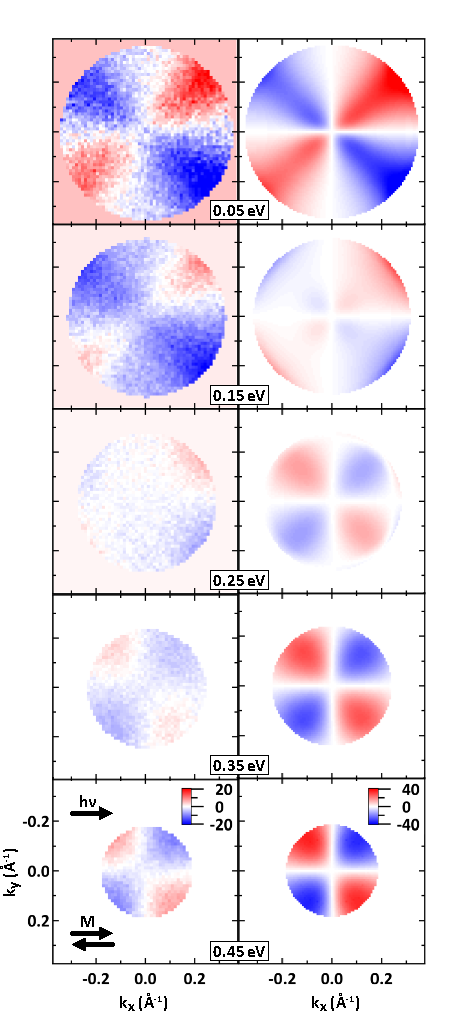
\includegraphics[width = 0.7\columnwidth]{FePaperApol.pdf}
    \caption{Momentum-resolved polarization asymmetry $A_{\mathrm{pol}}$ of Fe(001) at selected binding energies for 65° grazing light incidence. Left column: experimental results. The arrow marked $h \nu$ indicates the light incidence direction. The arrows $\textsf{M}$ represent the two magnetization directions considered for $A_{\mathrm{pol}}$. Right column: respective theoretical results obtained from photoemission calculations. The binding energy is indicated at each panel. The color scale, showing $A_{\mathrm{pol}}$ as defined in Eq.~\eqref{eq:Apol} in percent, is identical for all panels in this column. 
    }
    % Colorbar range in experimental Fe(001) A_pol data is always 40%.
    % The center position (white color value) is slightly adapted to the background such that the k_x=0 line is close to zero. This leads to the following five center positions (in %):
    % 	0.05 eV:    -6
    % 	0.15 eV:    -6
    % 	0.25 eV:    -1
    % 	0.35 eV:  -1.4
    % 	0.45 eV:  -1.5
    % Theory: Kinetic energies averaged +/-50 meV, T=0, 
    \label{fig:Apol}
\end{figure}

The theoretical pattern in the momentum space (right column in Fig.~\ref{fig:Apol}) exhibits a nodal line at $k_{y} = 0$ and almost a nodal line at $k_{x} = 0$. Moreover, one finds a change of sign if $k_{y}$ is reversed. These features are imposed by the symmetry of the setup. Note that an anti-symmetric pattern with respect to the $k_{x} = 0$ \textit{and} $k_{y} = 0$ lines follows strictly only for normal light incidence \cite{schumann2024}. However, the breaking of the anti-symmetric behavior with respect to the $k_{x} = 0$ line due to the off-normal light incidence is only hardly visible. The experimental data (left column) display the same features and the overall agreement between experiment and theory is remarkably good, which includes also the sign change for binding energies above and below 0.2\,eV. Note that the experimental asymmetries have been determined from two independent sets of 2D momentum maps for magnetization directions $+\vec{M}$ and $-\vec{M}$ oriented along the +x and -x directions, respectively, via selection of appropriate individual magnetic domains.

The momentum-dependent exchange asymmetry $A_{\mathrm{ex}}$, defined in Eq.~\eqref{eq:Aex} and shown in Fig.~\ref{fig:Aex}, exhibits absolute values up to $\unit[10]{\%}$ in theory and $\unit[6]{\%}$ in experiment, which are an order-of-magnitude stronger effects than previously observed \cite{marx2000}. An odd symmetry of the momentum-dependent $A_{\mathrm{ex}}$ pattern with respect to the $k_{x} = 0$ line would be expected for normal light incidence \cite{schumann2024}. However, for the grazing light incidence here, we find a clear deviation, which results in a curved nodal line between the regions of positive and negative $A_{\mathrm{ex}}$. With respect to the $k_{y} = 0$ line, both experiments and theoretical calculations show a mirror-symmetric pattern in contrast to $A_{\mathrm{pol}}$. The absolute $A_{\mathrm{ex}}$ values, including the sign, depend on the initial state binding energy via the band structure and photoemission matrix elements.

\begin{figure}
    \centering
    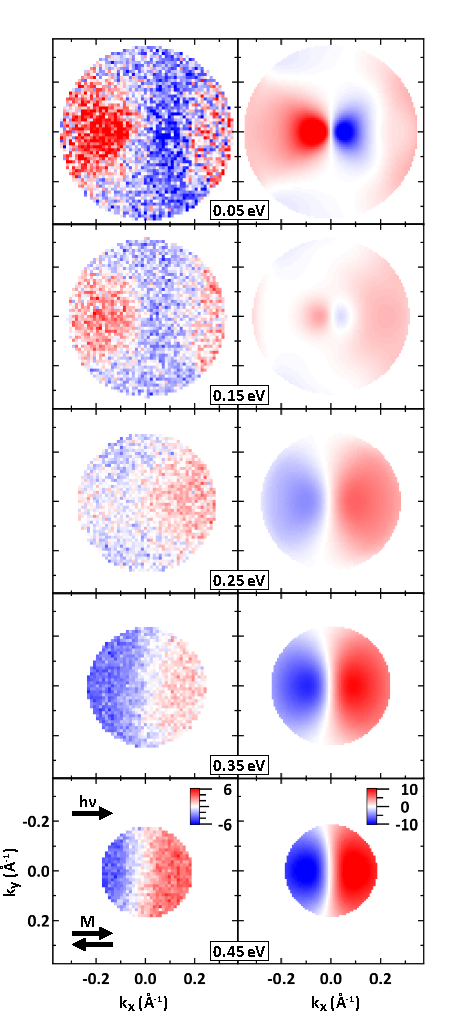
\includegraphics[width = 0.7\columnwidth]{FePaperAex.pdf}
    \caption{Momentum-resolved exchange asymmetry $A_{\mathrm{ex}}$ of Fe(001) at selected binding energies, as in Fig.~\ref{fig:Apol}. Left column: experimental PEEM data, right column: respective data from  photoemission calculations. Small differences with respect to an odd symmetry upon reversal of $k_{x}$ result from grazing light incidence. For normal incidence they are absent.}
    % Colorbar range in experimental Fe(001) A_ex data is always 12%.
    % The center position (white color value) is slightly adapted to the background such that the k_x=0 line is close to zero. This leads to the following five center positions (in %):
    % 	0.05 eV:  12
    % 	0.15 eV:  27
    % 	0.25 eV:   0
    % 	0.35 eV:   0
    % 	0.45 eV:   0   
    \label{fig:Aex}
\end{figure}

The above findings support that both asymmetries $A_{\mathrm{pol}}$ and $A_{\mathrm{ex}}$ are suitable tools for disentangling and quantifying the main contrast mechanisms for domain imaging. 

% \paragraph{Domain imaging.} 
From the momentum-resolved $A_{\mathrm{ex}}$ pattern in Fig.~\ref{fig:Aex}, it follows that MCD imaging can selectively reveal strong magnetic contrast in case of \emph{off-normal} electron momentum selection. However, without momentum selection or with a momentum selection centered at $k_x = k_y = 0$, which has been conventionally applied in the literature, different momentum contributions will largely cancel each other. This cancellation explains the small or vanishing magnetic dichroism for in-plane magnetized domains reported so far.

Our joint experimental and theoretical study suggests to selectively choose the $\vec{k}_{\parallel}$ area of interest in order to enhance the magnetic contrast. Hence, we place a circular contrast aperture in a $\vec{k}_{\parallel}$ area with high exchange asymmetry, a procedure known as dark-field imaging in optics and modern electron microscopy. 

Depending on the position of the aperture the contrast of specific domains is increased, as we show for a Landau-like pattern of four orthogonal magnetic domains at a Fe(001) surface. (Fig.~\ref{fig:Imaging}). Placing the aperture in nine different positions (black circles in the top panel of Fig.~\ref{fig:Imaging})  results in nine corresponding MCD PEEM images of the same surface region (bottom panel). 

\begin{figure}
    \centering
    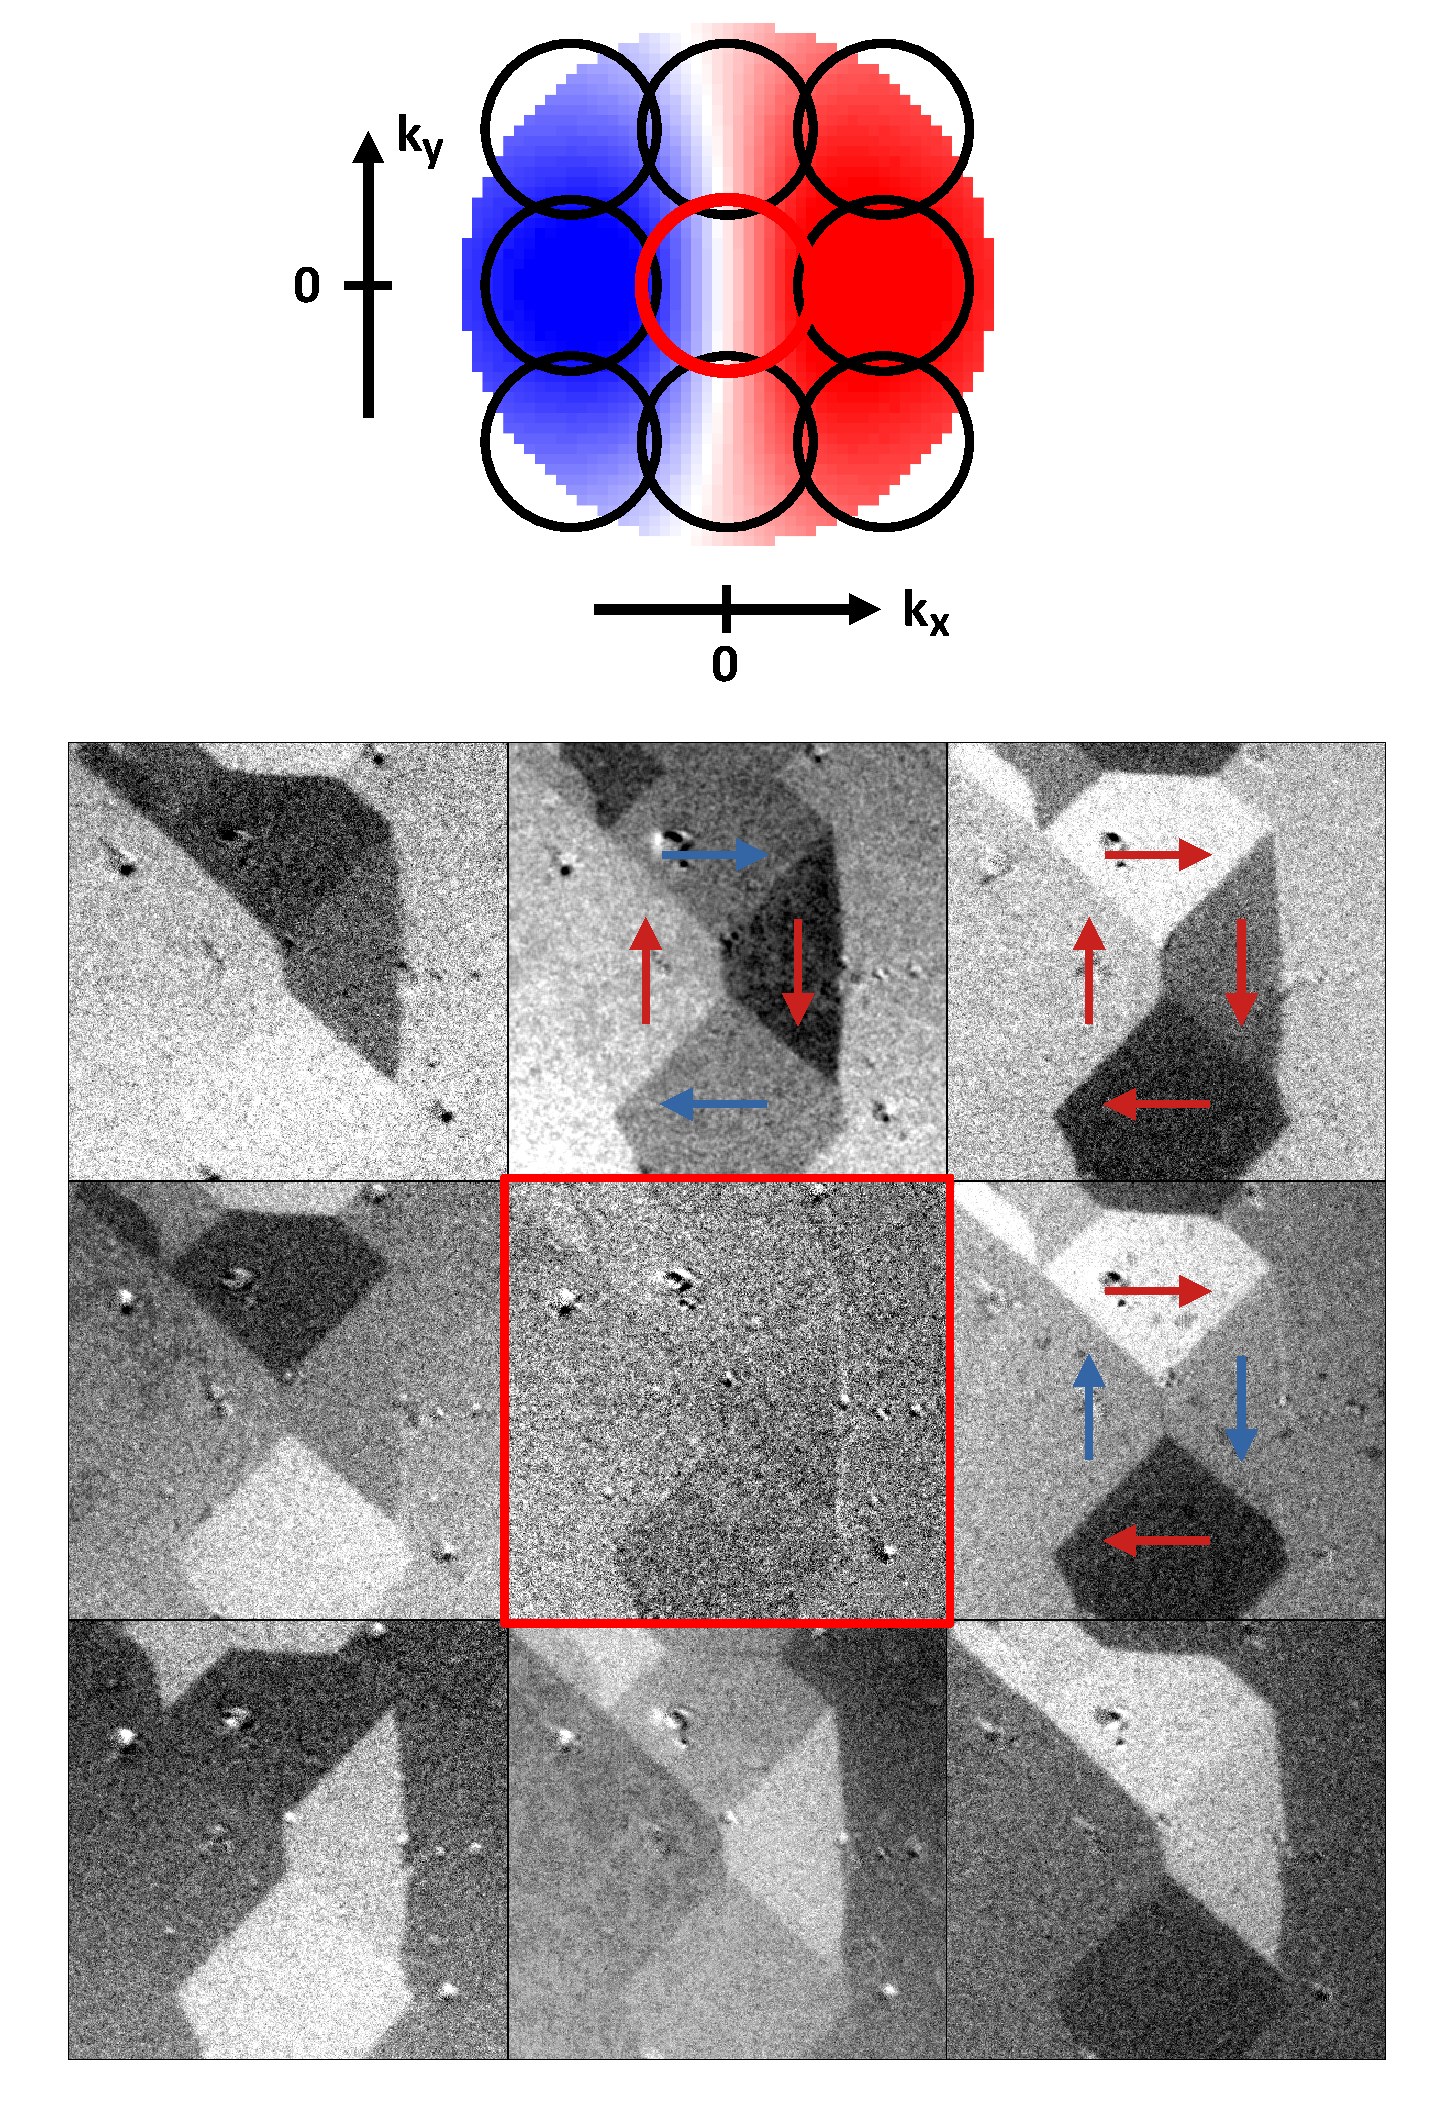
\includegraphics[width = 0.7\columnwidth]{FePaper9FelderSchema.pdf}
    \caption{Darkfield MCD imaging of Fe(100). Top: Schematics of the nine aperture positions in the momentum plane, with a momentum-resolved $A_{\mathrm{ex}}$ pattern as background. Bottom: Domain imaging using the nine aperture positions shown above. ($h \nu = \unit[5.2]{eV}$, 
    maximum domain contrast is between 3 and $\unit[4]{\%}$, field of view $56\times56\,\mu m^2$ each.)}
        % Positions of the momentum aperture (kx, ky) in $\AA^{-1}$:
        %       (aperture radius = 0.3)
        % upper left (-0.27, 0.17)
        % left       (-0.22, 0)
        % lower left (-0.21, -0.24)
        %     up         (0, 0.16)
        %     center  (0.03, -0.02)
        %     down       (0, -0.24)
        % upper right (0.39, 0.26)
        % right       (0.35, 0)
        % lower right (0.34, -0.26)  
        %
        % Binding energy range: between 0 and 0.8eV integrated 
    \label{fig:Imaging}
\end{figure}

For the centered aperture, marked in red, the MCD contrast almost vanishes in accordance with our above discussion. However, an aperture centered at $k_x > 0$ and $k_y = 0$ results in a drastically increased contrast of $\unit[3-4]{\%}$ for magnetic domains oriented in $+x$ versus $-x$ direction, whereas the contrast for domains oriented in $+y$ and $-y$ directions (blue arrows) vanishes. Both observations match quantitatively the result of the $\vec{k}_{\parallel}$ space measurements in Fig.~\ref{fig:Aex}. 

Positioning the momentum aperture at $k_x < 0$ and $k_y = 0$ reverses the contrast of $+x$ and $-x$ domains. As expected, the contrast switches from sensitivity in $x$ direction to $y$ direction when positioning the aperture at $k_x = 0$ and $k_y > 0$ (upper-middle PEEM image in Fig.~\ref{fig:Imaging}). The upper-right measurement shows a diagonal position with $k_x > 0$ and $k_y > 0$, where the different contributions to the MCD signal are combined, resulting in four different asymmetry values for the four in-plane magnetization directions. Note that in the latter case also $A_{\mathrm{pol}}$ contributes besides $A_{\mathrm{ex}}$ to the domain contrasts. 

% \paragraph{Initial-state effects.} 
The magnitude of $A_{\mathrm{ex}}$ and, therefore, of the MCD contrast in PEEM for near-threshold photoemission depend on the initial-state energy, as is demonstrated in Fig.~\ref{fig:Aex}. $A_{\mathrm{ex}}$ reverses sign from up to $\unit[+6]{\%}$ slightly below the Fermi level to $\unit[-4]{\%}$ at $E_{\mathrm{B}} = \unit[0.45]{eV}$. 
As a second, magnetically similar system we studied the oxygen-passivated Fe(001)-(1$\times$1)-O surface with darkfield threshold PEEM, as described above. It yields very similar $A_{\mathrm{pol}}$ and $A_{\mathrm{ex}}$ patterns as those for bare Fe(001) (not shown here), which reverse sign at a binding energy of approximately $\unit[0.2]{eV}$. Momentum-selected $A_{\mathrm{ex}}$ data from momentum-resolved PEEM measurements on 
the two in $\pm$\,x direction magnetized domains are shown in Fig.~\ref{fig:AexContrast}(b) for positive $k_x$ as blue squares and for negative $k_x$ as red circles. 

Using an angle-resolved photoelectron spectroscopy (ARPES) setup described previously~\cite{gillmeister2018, gillmeister2020}, the magnetic circular dichroism is analyzed in an independent experiment with higher energy resolution for an $\unit[11]{nm}$ thick Fe(001)-(1$\times$1)-O thin film grown on MgO(001). For fully in +x or -x direction magnetized films, the exchange asymmetry $A_{\mathrm{ex}}$ is depicted in an energy vs momentum map in Fig.~\ref{fig:AexContrast}(a). Note that the acceptance angle of the ARPES spectrometer is limited to $\pm15$\textdegree. Both datasets show large $A_{\mathrm{ex}}$ values, which switch sign upon reversal of $k_x$. At the Fermi level and at $E_{\mathrm{B}} = \unit[0.45]{eV}$ we find strong contrast of about $\unit[5]{\%}$ between $A_{\mathrm{ex}}$ values of +2 and $\unit[-3]{\%}$ with a contrast reversal between 0.15 and $\unit[0.25]{eV}$. We recall that this observation calls for exact threshold photoexcitation or for an energy-resolved electron detection in order to obtain high MCD signals. 
% Otherwise positive and negative exchange asymmetries will partly cancel each other.
This spectroscopic observations together with our microscopy data demonstrate that the full energy-momentum phase space of electronic states even for the paradigmatic system such as Fe can be fully utilized for magnetic dichroic domain imaging.

\begin{figure}
    \centering
    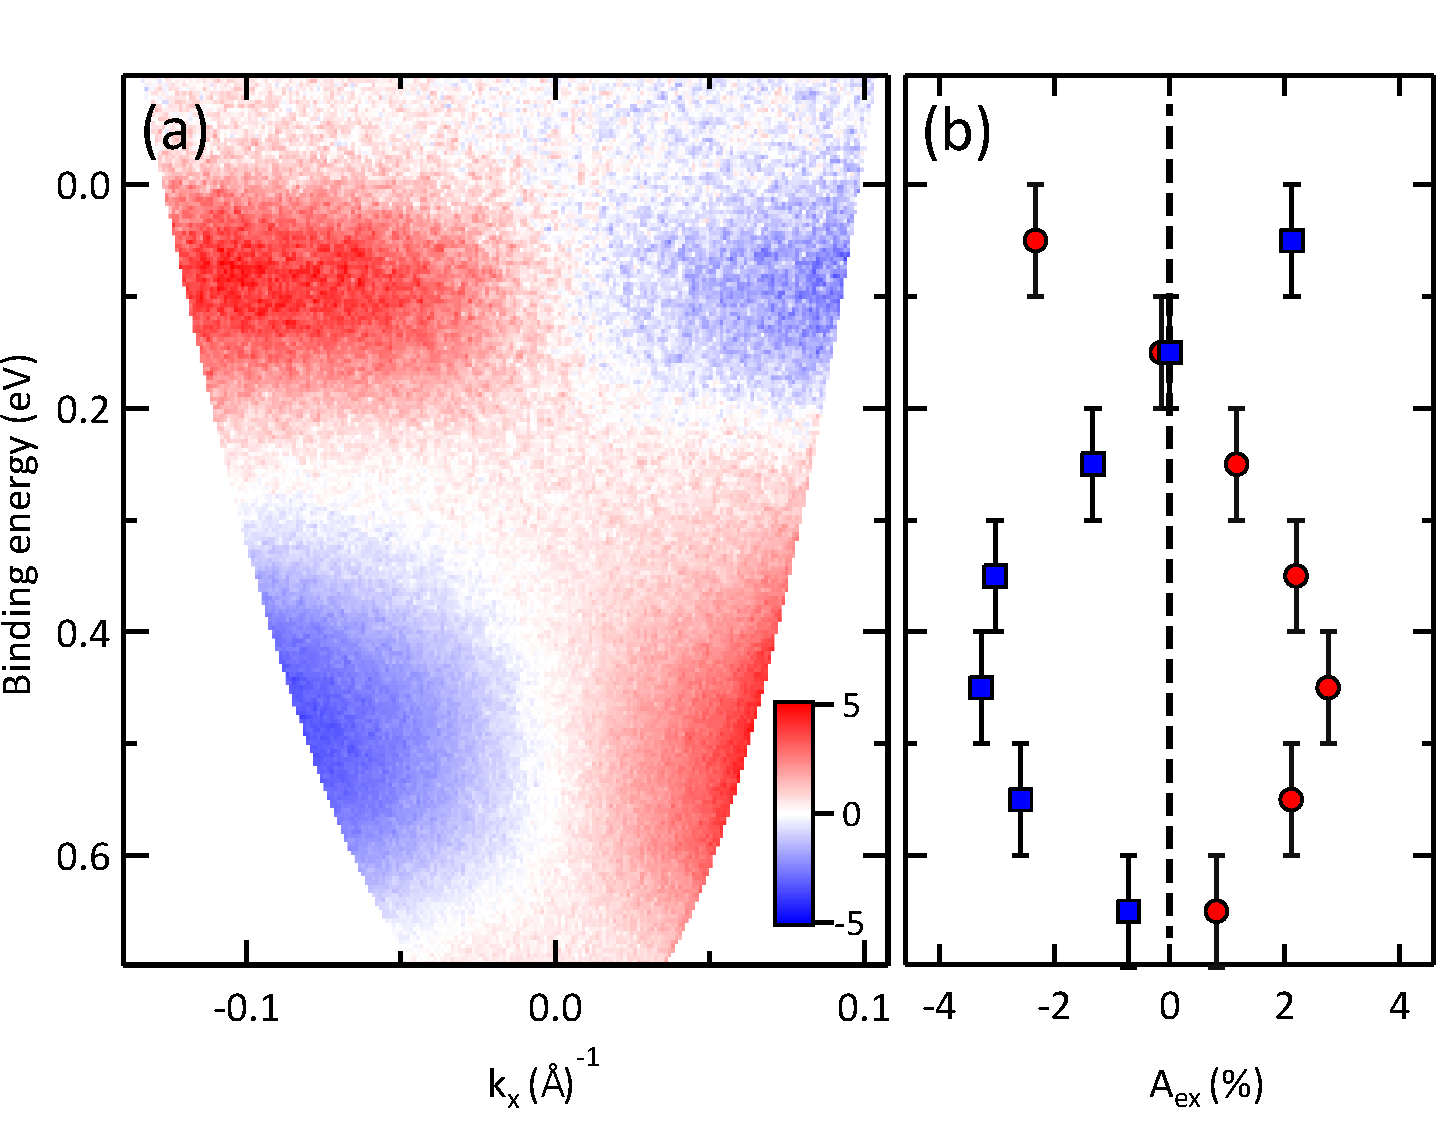
\includegraphics[width = 0.9\columnwidth]{FePaperFigARPES2.pdf}
    \caption{Binding-energy dependent exchange asymmetry $A_{\mathrm{ex}}$ for Fe(001)-(1x1)-O at $h\nu = \unit[5.2]{eV}$. (a) ARPES data for an oxygen-passivated Fe(001) thin film grown on MgO(001) with sample magnetized in $+x$ and $-x$ direction (light incidence at $\unit[70]{^{\circ}}$, $k_y = 0$). (b) Momentum-selected PEEM data for an oxygen-passivated Fe(001) single crystal for positive and negative $k_x$ momentum selection as marked by blue squares and red circles, respectively. (Selection at $|k_x| = \unit[(0.16 \pm 0.12)]{\text{\AA}^{-1}}$, $k_y = \unit[(0 \pm 0.12)]{\text{\AA}^{-1}}$, light incidence at $\unit[65]{^{\circ}}$).}
    % ARPES range of contrast in (a): 10% (-5 ... 5%) 
    % ARPES: $\Delta k_y = 0.001 \AA^{-1}$
    \label{fig:AexContrast}
\end{figure}

While the darkfield scheme of threshold MCD PEEM is broadly applicable, the magnitude of the binding-energy dependent exchange asymmetry $A_{\mathrm{ex}}$ is a material-specific property. It results from the spin-dependent electronic structure of Fe(001) and the associated ARPES  transition matrix elements. Note that for a fixed binding energy these matrix elements depend on the photon energy due to energy conservation.

% \paragraph{Summary and prospects.} 
This study demonstrates that magnetic domains can be imaged with high contrast using threshold PEEM with momentum selection of the detected photoelectrons, thereby introducing the concept of darkfield threshold MCD PEEM\@. We validated this approach by applying darkfield UV PEEM to an in-plane magnetized Fe(001) surface. However, this method is broadly applicable and can be extended to other ferromagnetic materials, including those with out-of-plane magnetization \cite{kronseder2011}, making it well-suited for investigating magnetic reorientation transitions, such as those observed in Ni/Cu(001) \cite{henk1999,sander2004,nakagawa2006,kronseder2011}.

The most promising potential of this technique lies in its ability to investigate ultrafast magnetization dynamics using femtosecond laser pulses in an optical pump and threshold UV photoemission probe scheme. This capability opens new avenues for studying the ultrafast motion of domain walls \cite{parkin2008} or large skyrmions on nanometer length scales \cite{goebel2019,jani2021,kern2022}.

\paragraph{Acknowledgments.} This work is funded by the Deutsche Forschungsgemeinschaft (DFG, German Research Foundation) -- Project-ID 328545488 -- TRR~227, projects~A06 and~B04.

% \bibliographystyle{}
\bibliography{references}

% \listoftodos

\end{document}
